%
% Titelseiten Datei
%

\begin{titlepage}

	% Fehler "destination with the same identifier" unterdr�cken...
  \setcounter{page}{-1}

	% Titelseite
	\begin{figure}[h]
		\begin{minipage}[b]{25mm}
			
\includegraphics[width=25mm,clip]{images/logo_uhh}
		\end{minipage}
		\begin{minipage}[b]{2mm}
			
\includegraphics[width=1mm,height=24mm]{images/greypixel}
		\end{minipage}
		\begin{minipage}[b]{12 cm}
			{\sffamily
				{\Large Hamburg University } \\
				Faculty of Mathematics,\\
				Informatics and Natural Sciences \\
				Department of Informatics \\
			}
		\end{minipage}
	\end{figure}

	\vfill
	
	\begin{center}
		% Diplomarbeit 
		\noindent { \huge
			Master Thesis \\
					}
		\vspace{14mm}
		% Titel
		\noindent \textbf{\Large
		  Incremental Speech Recognition from Several Combined Sources \\		  
		}
		\vspace{10mm}
		submitted on 04.09.2016
		\noindent {\large
		
		}
	\end{center}
	
	\vfill
	
	\noindent \textbf{Natalia Orlova} \\
	\noindent \rule{\textwidth}{0.4mm} 
	\noindent{\textrm{2orlova@informatik.uni-hamburg.de}} \\
	\noindent{\textrm{Degree Program: Master Informatics}} \\
	\noindent{\textrm{Matr.-No. 6459416}} \\
	%\noindent{\textrm{Fachsemester <XX>}} \\
	\begin{tabbing}
	\hspace{20em} \=  \kill
	First supervisor Hamburg University: \> Dr. Timo Baumann \\
	Second supervisor Hamburg University: \> Prof. Dr. Wolfgang Menzel \\
		
	\hspace{20em} \=  \kill
	
	%(Option)Betreuer <Firma>: \> <Vorname> <Name> \\
			
	\end{tabbing}
	
	% R�ckseite der Titelseite mit Zitat
	%\newpage 
	%\thispagestyle{empty}
	%\setcounter{page}{0}

	% wenn man Lust auf ein Zitat hat...
	% ... ansonsten auskommentieren
	%~\\ \vfill \noindent 
%	A distributed system is one where the failure of some \\
%	computer I've never heard of can keep me from getting my work done. \\
%	\textit{-- Leslie Lamport}
\end{titlepage}

%
% EOF
% 
\section{Introduction}
\subsection {Motivation}
In recent years, Automatic Speech Recognition (ASR) systems have improved
increasingly, being used in everyday applications: Siri, Google ASR 
\parencite {mcgrawgrauenstein2012}. However, most of such systems work
asynchronously in respect to output, computing the result after the utterance is already finished.
In the area of Human-Machine Interaction, 
where intermediate system reactions of ASRs are 
desirable,  incremental output of the intermediate results becomes increasingly
important. Benefits of  incremental speech recognition include post-processing
time savings, faster system feedback and more natural dialogue between humans
and intelligent systems. Commercial Google recognition
engine, working in incremental mode, produces accurate
results in non-specific domains, but demonstrates high latency \parencite{mcgrawgrauenstein2012}.  Non-commercial open source systems, like Sphinx-4, on
the other hand, demonstrate very short delays and can be timed to specific
applications, but are less reliable in accuracy.
The challenge is to combine the advantages of both systems and  to overcome the latency problem of Google-ASR.
\subsection {Problem Statement}
The aim of this master thesis is to investigate the possibility of
timeliness and timing improvement of Google ASR
incremental results by developing a state-of-the art 
combination of Google Incremental ASR \parencite {mcgrawgrauenstein2012} and an
incremental speech recogniser, based on Sphinx-4 \parencite
{baumannetal2009:naacl}. 
\subsection {Objectives}
% The aim of the master thesis is to improve the timeliness of incremental
% speech recognition by developing a state-of-the art 
% combination of Google Incremental ASR \parencite {mcgrawgrauenstein2012} and an
% incremental speech recogniser, based on Sphinx-4 \parencite
% {baumannetal2009:naacl}. The architecture of the incremental recogniser is shown in the Figure \ref {fig:Bild1}. The first aim is to get the
% detailed timing information for incremental Google-ASR results, using
% forced alignment technique. The second objective is to
% be able to reset the SearchGraph of the Sphinx-4 recogniser, by going back to
% the saved state and choosing an alternative path. The third central aim is to
% manipulate SearchGraph. Manipulation includes doing reset, depending on the
% timing information about forced-aligned phonemes, coming from Google ASR
% and changing the hypotheses path. Furthermore it should be able to make a
% combination of Google-ASR and Sphinx-4, using Google incremental output as a
% guidance for SearchGraph manipulation and hypotheses correction, when Google
% incremental output differs from Sphinx-4. 
The following objectives states, how the aim of the master thesis is going to be
addressed:
 \begin  {itemize}
   \item Forced-alignment of Google incremental results, using a
   combination Google and Sphinx ASRs
   \item Evaluation of timing results, comparing Google alone, Sphinx alone and
   Google + Sphinx combination, using evaluation metrics
   \item Overcoming of Google latency in a combined Goole + Sphinx ASR, by
   investigating the possibility of Sphinx SearchGraph reset and changing the
   hypotheses path 
   \item Evaluation of timeliness results, comparing Google alone, Sphinx alone
   and Google + Sphinx combination, using evaluation metrics
 \end {itemize}

%  \begin{center}
% \begin{figure}[htbp]
%   \centering
%      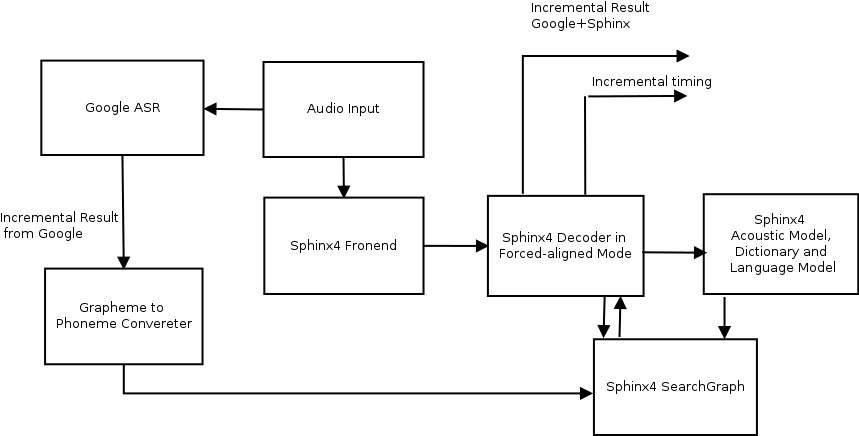
\includegraphics[width=0.9\textwidth]{images/overview.png}
%   \caption{Incremental recogniser from combined sources}
%   \label{fig:Bild1}
% \end{figure}
%  \end{center}
% The final objective is to evaluate and to visualize timeliness  of the
% implemented incremental recognizer, using a combined technique in comparison
% with Google-ASR system or Sphinx-4 based system alone.
\subsection {Structure}
This expos\'{e} is structured as follows. Section 2 provides review of 
scientific papers, related to the thesis topic. %Section 3 is a brief statement
%of the research questions. 
Section 3 presents an example to illustrate the
problem of Google ASR timing. Section 4 contains methods to be used for this
research.
Section 5 describes the evaluation approach and expected results. Section 6
contains preliminary table of contents for the upcoming thesis. In the section 7
a timeline for the thesis is presented. Section 8 summarizes the expos\'{e}.

\section {Related Work}
The architecture of  contemporary speech recognition systems includes basic ASR
components: acoustic input, acoustic model, language model and decoder.
ASR decoder gets as input feature vectors of audio signal and the results
of acoustic and language modelling and produces a decoded word and
phone alignment as an output \parencite {jurafskymartin2009}.

Most traditional ASRs, including commercial, are not incremental. They produce
the output result after the utterance is finished, resulting in a delay up to
750-1500 ms. In additional they may use multiple-pass decoding, which is not
possible incrementally \parencite {skantzeschlangen2009}.
Incremental dialogue processing allows reducing of feedback time, bringing the
dialogues in interactive environments closer to natural ones.
Apart from abstract models of incremental dialogue processing there exist an
implementation  of a limited micro-domain system, recognising sequence
numbers \parencite {skantzeschlangen2009}.

A good example of  traditional ASR architecture is the implementation of the
open-source CMU Sphinx-4 recogniser \parencite {Lamereetal2013:Eurospeech}.
Sphinx-4 was not designed as an incremental system, but its modular design 
allows extension and adding new components, required for an incremental speech recogniser. 
\parencite {baumannetal2009:naacl}.

Apart from Sphinx-4 the leading speech recognition systems is commercial
Google Voice Search \parencite{schalkwyk2010}.

State-of-art Google Search by Voice, trained using huge amounts of audio data,
presents the best results in the terms of accuracy for a
standard non-incremental task. However, when intermediate results are produced
synchronously in an incremental mode we see a trade-off between stability of the
input and latency \parencite {mcgrawgrauenstein2012}. 

Further restriction of Google is its task-orientated recognition, primarily 
aimed to interactive Google command search. This generally means that simple
transfer of Google technology to domain-specific natural dialogue systems and
context-specific HRI environments leads to lower accuracy. 

Recently, there has been proposed a solution for a domain-dependent
applications, using a combination of Google phonetic post processing and
Sphinx-4. Original frontend of Sphinx-4 is replaced by phoneme frontend, which
converts the Google result to its phonetic representation. Test
results of the combined approach have shown a significant improvement of
recognition results for non-incremental tasks.
Combination technique is considered to be transferable to the
incremental problem solution \parencite {twiefeletal2014}.

% \section {Research Question}
% As already stated above the main research question of the master thesis is
% timing and timeliness improvement of an incremental speech recogniser,
% implementing forced alignment of Google incremental results, Sphinx searchGraph manipulation and developing a combination of Google
% ASR and Sphinx-4 recogniser (cmp.\cite {twiefeletal2014}).
% 
% As in incremental recogniser intermediate results are produced while the speaker
% has not yet finished the utterance, the focus of the research becomes detailed
% timing of input and output. Monitoring of its own input in relation to output is
% a crucial point for a system to be able to revoke or commit the state of the
% recogniser \parencite {skantzeschlangen2009}.
% 
% Under the above considerations, we are dealing with the
% following research subquestions. The first problem is forced alignment of
% Google incremental results with audio input. The idea is to
% get an accurate timing information for Google incremental results and to improve
% in such a way the existing Google timing. For calculating of the actual timing
% standard deviation and nets latency are to be taken into account. Second problem is 
% studying the possibility of Sphinx SearchGraph manipulations and hypothesis path reset 
% within schinx4. Third problem is improvement of Sphinx recogniser performance
% by combining Sphinx and Google.


\section {Example to Illustrate the Timing Problem of Google ASR}
In the following section a simple example is provided to sketch the problems to
be researched in the master thesis. For this example  a simple audio file
'DE$\_$$1234$.wav' is used, where the numbers 1-2-3-4, pronounced one after
another in German language, are recorded. 

Picture \ref {fig:Bild2}  visualizes time alignments, created manually
(transcription '.manual') and with the help of existing forced alignment module
(transcription '.sphinx'), implemented in Inprotk, using sphinx4 recogniser
alone. Incremental results, coming direct from Google with particular network
latency, contain only information about hypotheses timing. Transcription .google
shows forced alignment, applied to Google results and calculated
by the existing time-alignment module \parencite {baumannetal2009:naacl}.  As it
can be seen from the picture the alignment of the sphinx approximates the true
alignment, whereas the timing, calculated for Google, is not only delayed by the
net latency, but also incorrect in duration. 

 \begin{figure}[htbp]
  \centering
     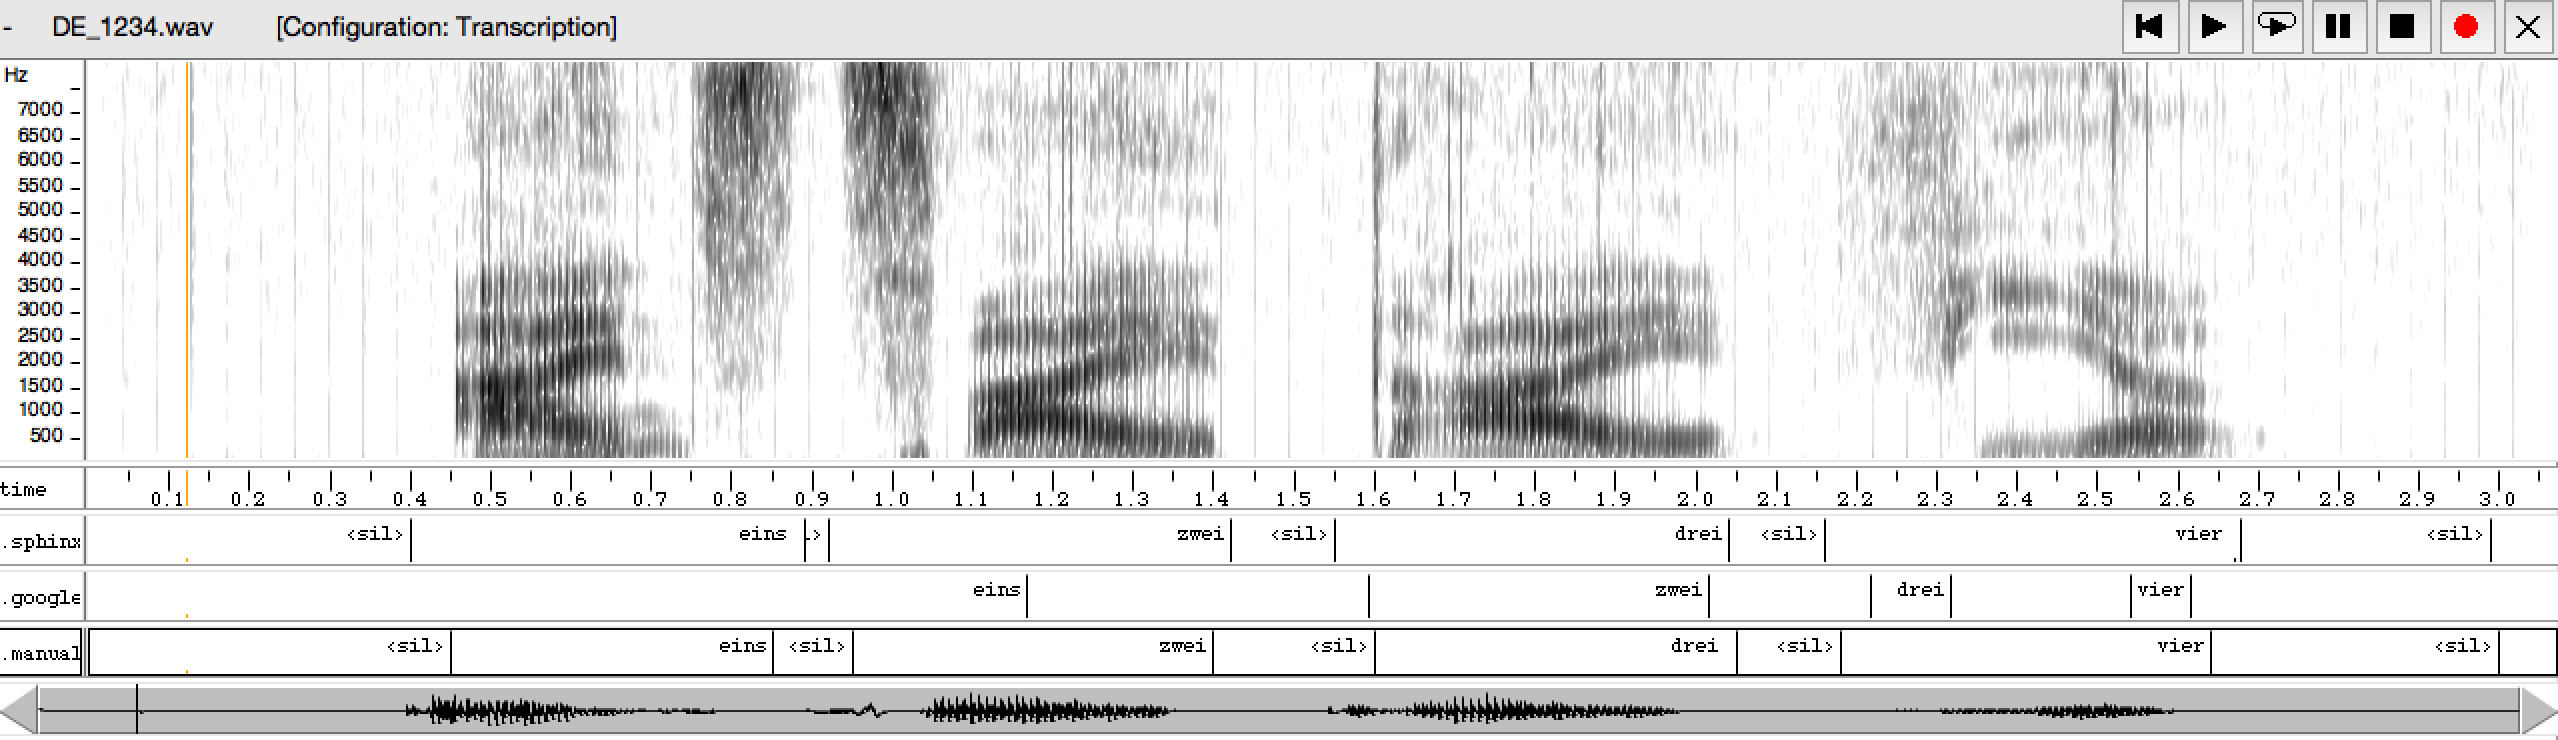
\includegraphics[width=1.0\textwidth]{images/wave2.png}
  \caption{Audio Input Alignment}
  \label{fig:Bild2}
\end{figure}

% Pictures   \ref {fig:Bild3} and  \ref {fig:Bild4} show the incremental output
% of both ASRs: sphinx4 and Google in detail. This pictures also illustrate 
% that outputs differs not only in the number of hypotheses and  nets latency
% time.  
% \begin{figure}[htbp]
%   \centering
%      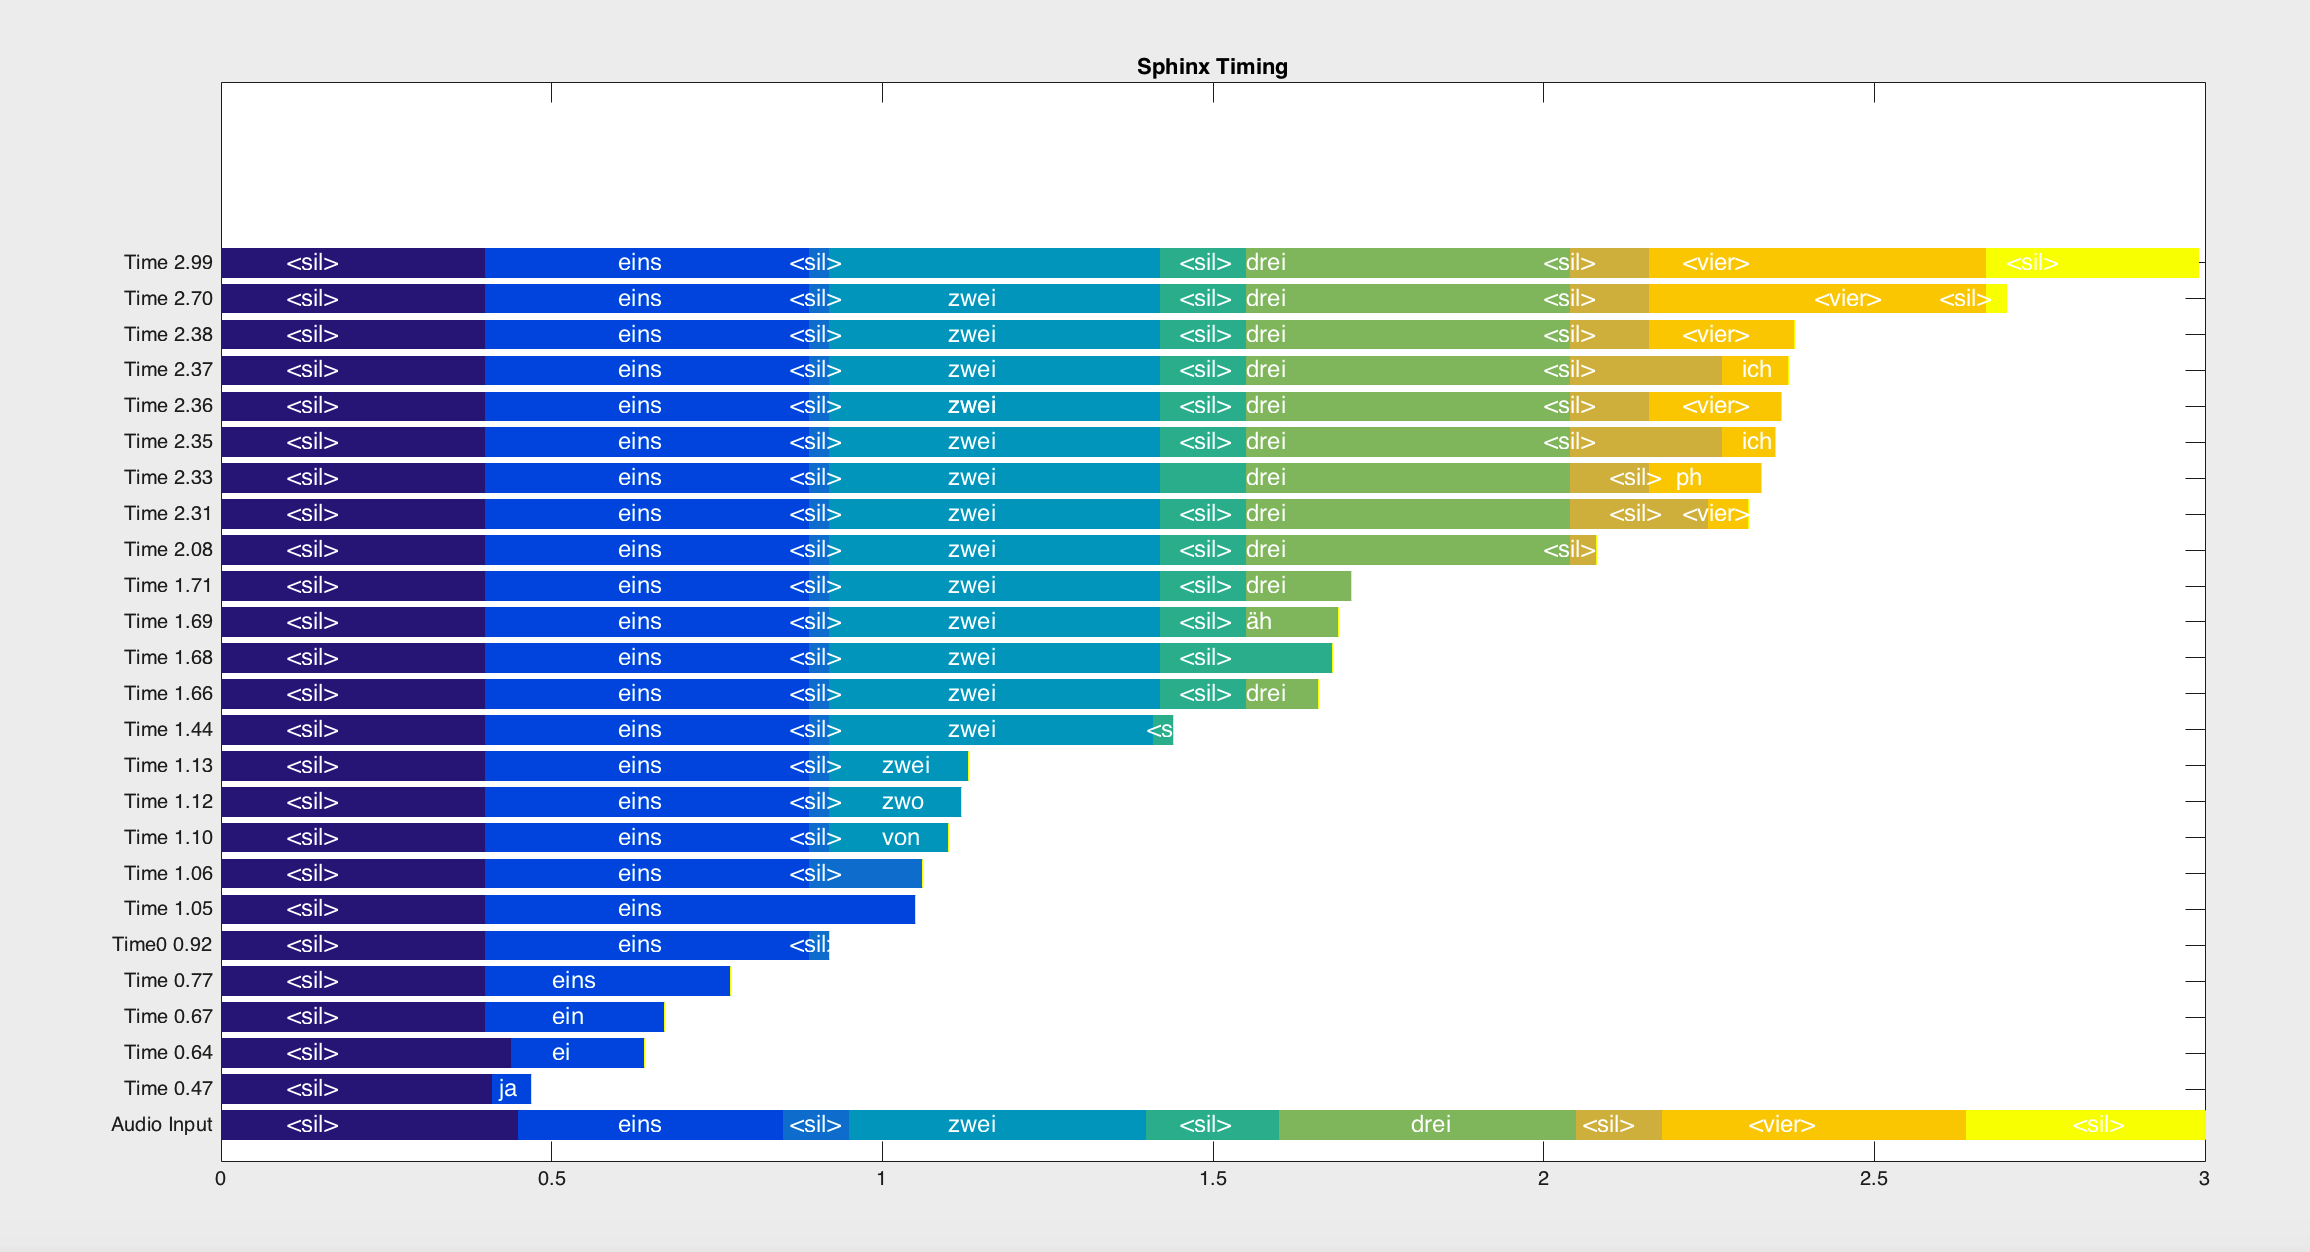
\includegraphics[width=1.0\textwidth]{images/SphinxTiming.png}
%   \caption{Audio Input and Sphinx Recognizer Timing Visualisation}
%   \label{fig:Bild3}
% \end{figure}
% 
% \begin{figure}[htbp]
%   \centering
%      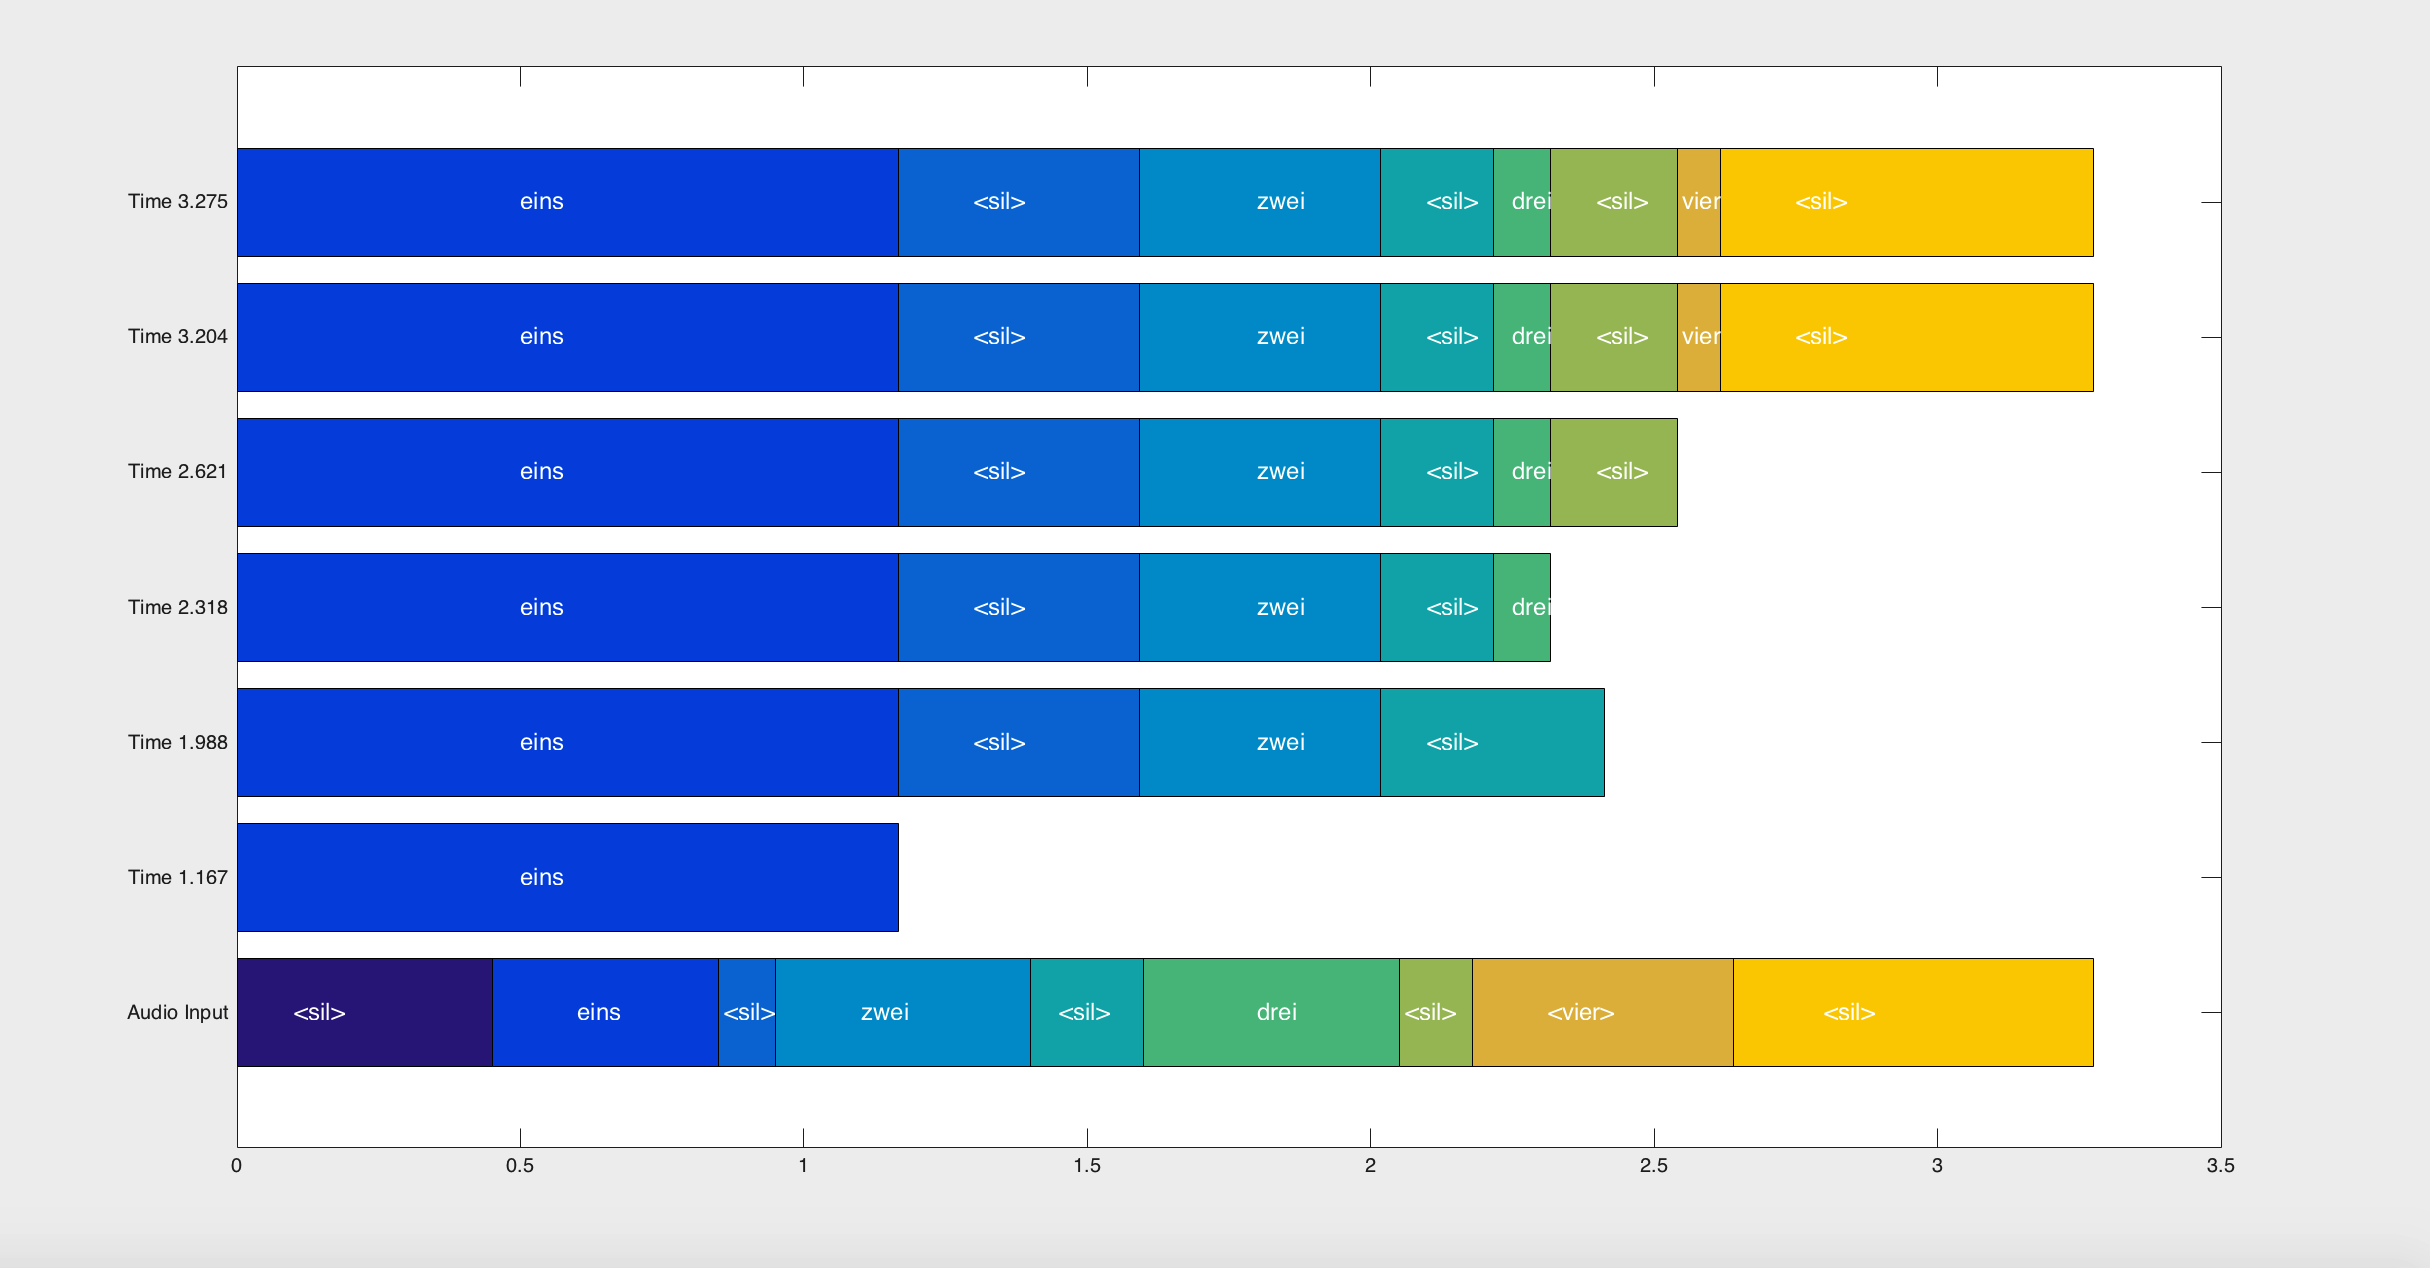
\includegraphics[width=1.0\textwidth]{images/googletiming.png}
%   \caption{Audio Input and Existing Google Recognizer Timing Visualisation}
%   \label{fig:Bild4}
% \end{figure}
The difference between Google timing  and true
alignment is not always constant. For example, if we calculate the mean fault
between Google timing and true timing with the formula:
%$\frac{Delay-True\;Timing}{Number\;of\;Word\;Matches}$ 
$mean\; fault=\frac{\sum_{n=0}^N Delayed
Timing-True\;Timing}{N \;of\;Word\;Matches \;and\;Substitutions}$ the
corrected timing still does not correlate with the gold manual transcription.
Apart from the delay an incorrect word duration is also observed. The results of
the mean fault correction are shown in the picture \ref {fig:Bild5} (transcription .mean).
\begin{figure}[htbp]
  \centering
     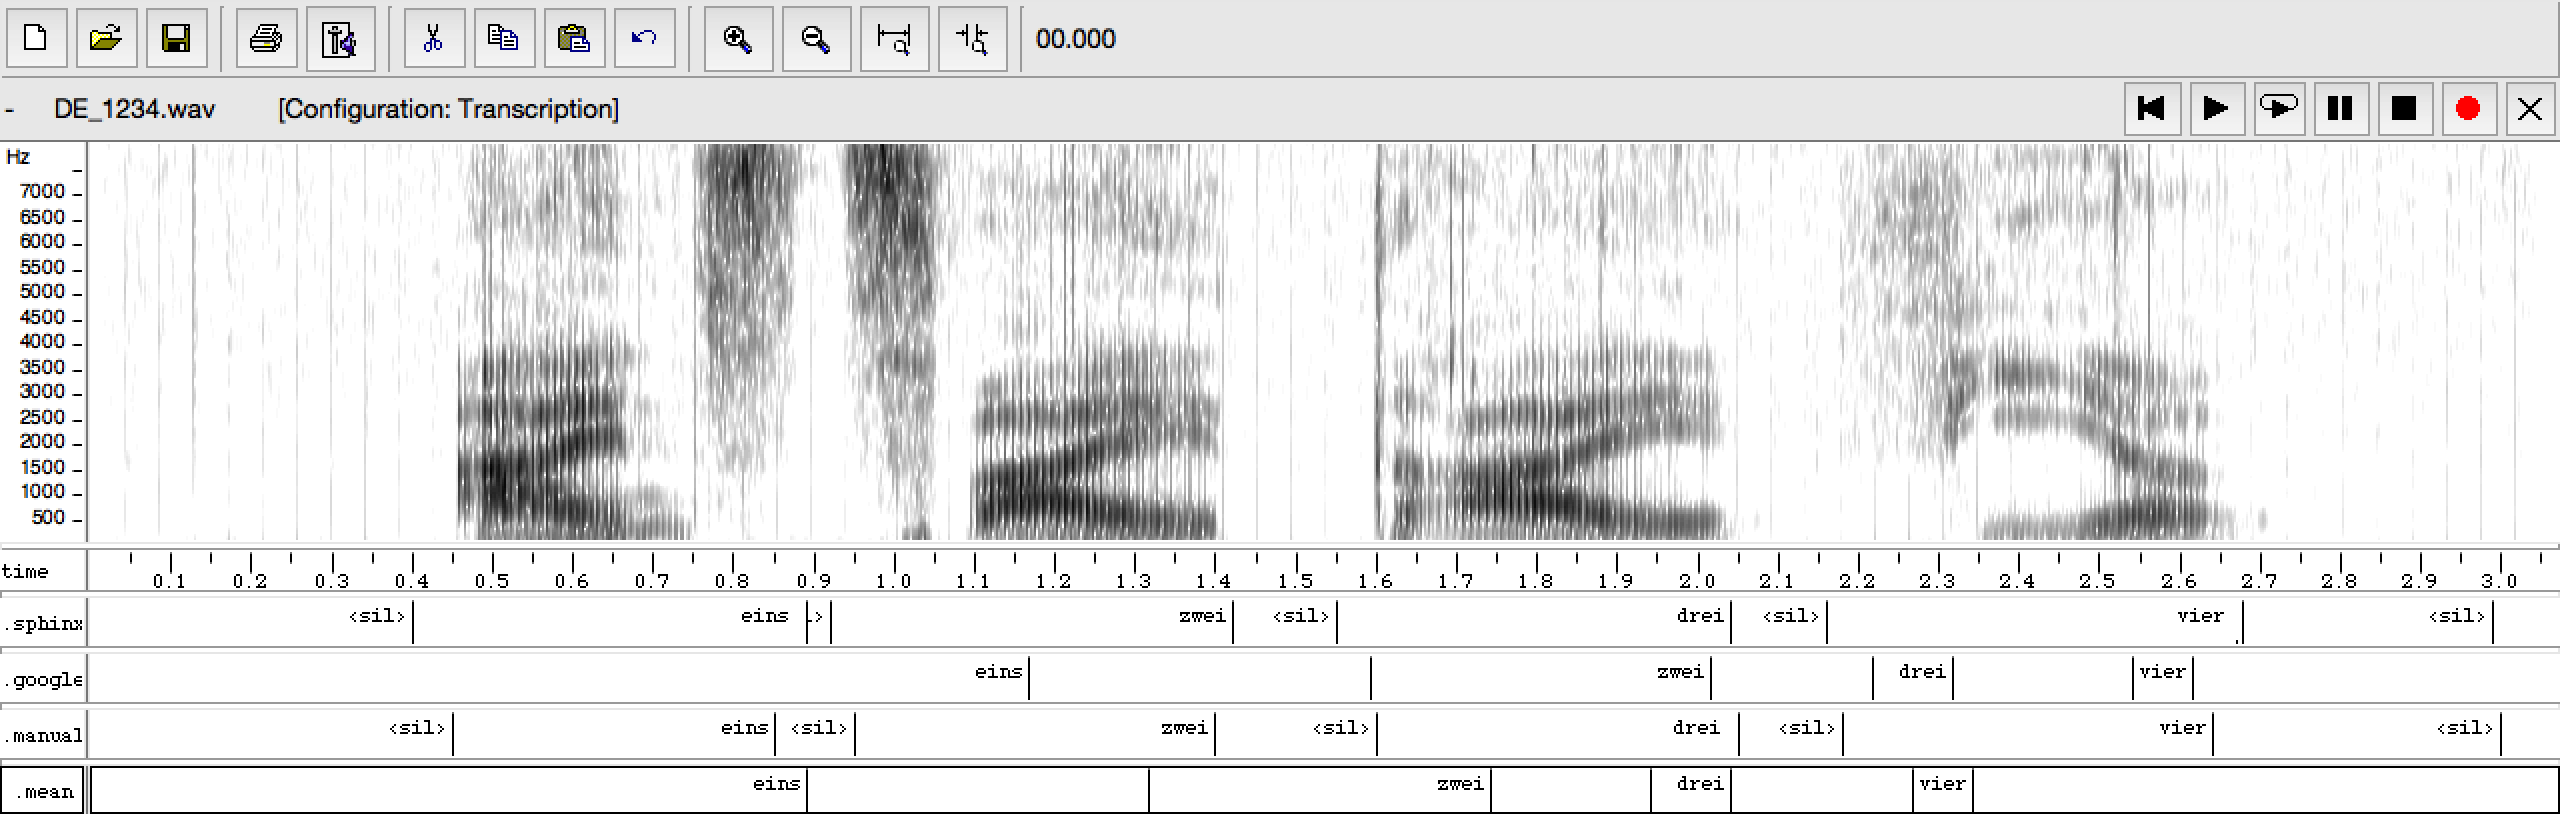
\includegraphics[width=1.0\textwidth]{images/wave3.png}
  \caption{Audio Input Alignment and Mean Fault Correction for Google Results}
  \label{fig:Bild5}
\end{figure}
To implement the forced alignment for Google ASR several facts are to be
considered. First, we are dealing with the network latency. 
Second it is not enough to correct the result by a constant factor as the
standard deviation of hypotheses output, produced by Google, should also be taken into account. 
Timing, giving information about alignment of Google incremental output
to audio input will be further used to manipulate the SearchGraph of the
sphinx4.

\section {Methods}
\subsection {Development Environment}
Incremental recogniser will be implemented in Java programming language, using
an open-source project Incremental Spoken Dialogue processing
Toolkit (InproTK), developed by the Universities of Potsdam, Bielefeld and
Hamburg. InproTK includes modules for speech recognition, speech understanding,
speech processing and dialogue management.
Speech recognition module is based on implemented Java Sphinx-4 recogniser, a
package of CMUSphinx speech recognition toolkit. 

\subsection {Data Structures}
Incremental Recogniser architecture includes Sphinx-4 Frontend, Dictionary,
Language Model and Acoustic Model, Decoder in forced-aligned mode,
SearchGraph (see Figure \ref {fig:Bild1}).
\begin{center}
\begin{figure}[htbp]
  \centering
     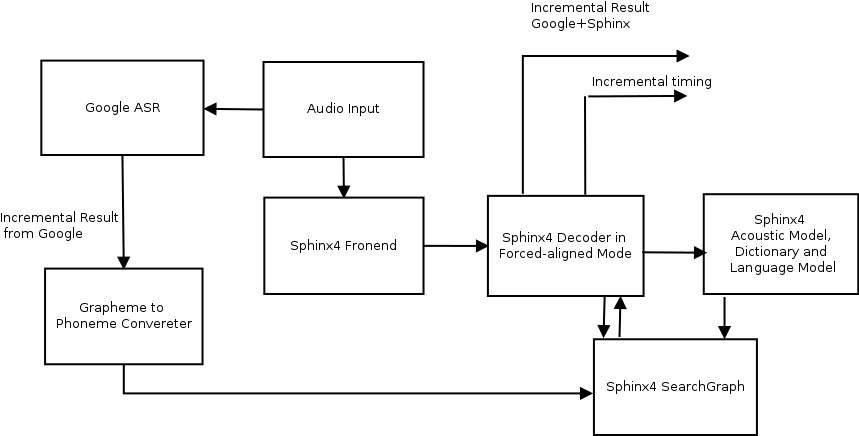
\includegraphics[width=0.9\textwidth]{images/overview.png}
  \caption{Incremental recogniser from combined sources}
  \label{fig:Bild1}
\end{figure}
\end {center}
\subsubsection {Audio input}
As an audio input both Google and Sphinx receive the same audio files. Google
will use the audio input for recognition. Sphinx will use the audio input
for alignment of Google incremental results as well as for recognition.  
\subsubsection {Frontend}
Frontend computes feature vector representation of speech signal, using acoustic
analysis. For this master thesis a standard Sphinx-4 frontend is to be used as a
Frontend. It provides methods for manipulating the processors, performing
specific transformation functions on input data \parencite{Lamereetal2013:Eurospeech}.
\subsubsection {Acoustic Models and Hidden Markov Model}
Acoustic model finds out the probability for an observing an acoustic vector Y
given a sequence of words P(Y|W). For a small vocabulary it can be found by
sampling several variants of the words and computing statistical similarity of the inputs with the existing
samples. However, when the vocabulary is very large we have to move down to the level of word
subunits or phonemes.
Acoustic model contains statistical representation of each phoneme in the form a Hidden
Markov Models (HMM), which abstracts the physical process of pronouncing of a
particular phoneme. In order to get
a statistical representation of phonemes, i. e, build an automate with
transition probabilities for each phoneme, the speech corpus data is subjected
to the training process.
\parencite {jurafskymartin2009}.
\subsection {Language Model}
Language model describes the probability of a word in a speech sequence P (W)
and attempts to predict the next word in a sentence, depending on the prior context.
Language models are based on n-gram sequences of words, where the number of words of
the prior context is equal n-1. Language models are built on the basis of an
application corpus \parencite {jurafskymartin2009}. Depending on the
application, language models can be either generalized or domain specific. 
\subsubsection {Decoder and SearchGraph}
On the basis of acoustic model, language model and dictionary the SearchGraph
is build, which is used by the decoder together with the frontend information
to determine the most probable output sequence. Decoder
traverses the network of HMM states and finds the path with the best
score, using Viterbi algorithm. 
\subsubsection {Grapheme to Phomene Converter}
Grapheme to phoneme converter converts  a sequence of character strings into a
sequence of phones, according to the international phonetic alphabet  standards.  
Sphinx provides grapheme to phoneme conversion feature as a part of its
implementation \parencite {Lamereetal2013:Eurospeech}.
\subsubsection {Time alignment Component}
Timing component, which is to be implemented as an
Incremental Unit (IU), forwards the incremental Google results for further
alignment to Sphinx ASR. It is supposed to ensure buffering and updating of
audio input, related to partial incremental results.
% timing information Google incremental
% result. 
% Time alignment component computes alignment of Google incremental results with
% respect to audio input. Furthermore timing is intended to manipulate the
% SearchGraph. Manipulation includes reset, allowing back tracking to the saved
% state and changing the search path in the graph.
\subsubsection {Google-Sphinx Combination}
The implementation of the incremental speech recogniser is to be realised as a
combination of Google ASR and Sphinx recogniser. 
% , whereas the states of the
% Search-Graph are manipulated, depending on the incremental output, coming from
% Google.  
Frontend, Acoustic model, Dictionary and Linguistic Model are chosen from
the standard ones, offered by Sphinx. 
%Google incremental
% results are preprocessed in the grapheme to phoneme converter and undergo forced
% time-alignment. 
The initialisation and implementation of the SearchGraph is realised by
Sphinx-4. The choice and alternation of the path in
the SearchGraph depends on the Google incremental hypotheses. 
When the new Google hypotheses differs from the present hypotheses in the
SearchGraph, the SearchGraph is reseted and the hypotheses path is
corrected.  Timeliness improvement is supposed to be achieved by faster results
produced by Sphinx, whereas the path in the Sphinx SearchGraph is predetermined
by Google incremental result. The last means that we get the same final results
for Google and Google + Sphinx, but timeliness of Google + Sphinx
is expected to be improved. 
%Furthermore an alternation between single Google-ASR, single
%Sphinx-4 and a combination of Google-ASR and Sphinx-4 is foreseen.
\subsection {Algorithms} 
\subsubsection {Viterbi search algorithm}
Search in the Sphinx-4 decoder module is executed, using Viterbi algorithm
\parencite {Lamereetal2013:Eurospeech}.
Viterbi is a dynamic programming search algorithm. It traverses the network of HMM states and finds the
path with the best score. Abstract representation of the Viterbi algorithm is
shown in the in the figure \ref{fig:Bild6}. One axis represent states in the
HMM network, another time. Arrows means transitions through the network. Each point in this 2-D space represents the best path probability for the corresponding
state at that time. Every state has a best predecessor and starting from the final state and
using backtracking it is possible to find the best path sequence for the whole
search.
\begin{figure}[htbp]
  \centering
     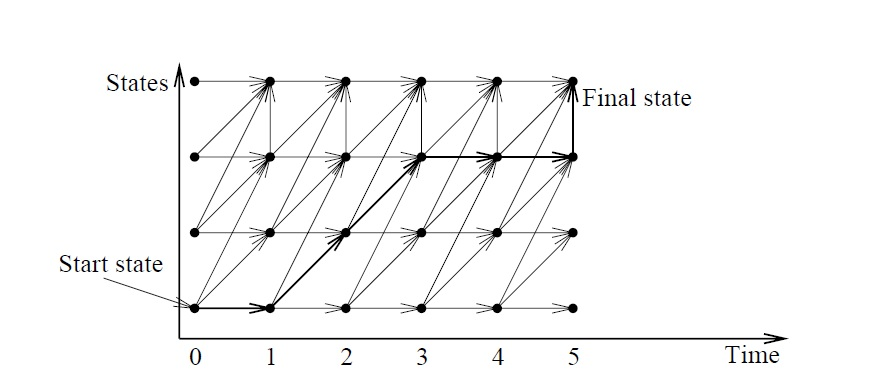
\includegraphics[width=0.9\textwidth]{images/viterbi.jpg}
  \caption{Viterbi Search algorithm \parencite {jurafskymartin2009}}
  \label{fig:Bild6}
\end{figure}

\subsubsection {Similarity Metric and Levenshtein Distance }
Leveshtein distance is a similarity metric of two stings. Levenshtein distance
algorithm calculates a Levenshtein distance matrix, containing substitutions,
matches, deletions and insertions of characters, occurring in two strings
\parencite {levenshtein1966}.  
% % Each
% substitution increases Levenstein distance by 1 
% . Timing difference will be calculated only for matches and
% substitutions of audio transcription and Google incremental results.
\subsection {Test Data} 
For testing purposes  a corpus of  a total of 27 hours of audio files  is
available.  Each record contains audio file, true alignment and Google
incremental results in JSON format, including hypotheses timing.  For
development purposes a smaller part of this data, consisting of 30 audio files, is to be used. For validation purposes corpus will be
gradually extended with additional data. 
\section {Evaluation Approach and Expectations}
For results evaluation evaluation library InTELiDa (Incremental Timing
Evaluation of Linguistic Data), providing a graphical user interface for
incremental data analysis, will be used \parencite {baumann2013:phd}. 
The results for Google alone, Sphinx alone and Google + Sphinx are to be
compared. Timing for each recogniser is to be evaluated using mean error, root
mean square error for matches and substitutions, whereas timing results of
each recogniser is to be compared with the gold standard. 
Approach, used for timeliness evaluation, is similar in the choice of the
recognisers to be compared. The difference is that in the case of
timeliness First Occurrence (FO) and Final Decision (FD) metrics are used. 
The  timing and timeliness results of Gooogle + Sphinx combination are
expected be better than the results of Google ASR and Sphinx ASR alone.

%In the chapter the quality and performance of the implemented Incremental
% Speech
% recogniser is to be analysed. As a metric for performance analysis latency time
% is to be used. Latency is understood here as the time difference between audio
% incremental input and incremental output of the recogniser.  Latency of Google
% ASR, Sphinx-4 based recogniser alone and a Coogle-Sphinx combination are supposed to be computed
% and visualises graphically, showing the delays for single incremental
% results. For this purpose evaluation library InTELiDa (Incremental Timing
% Evaluation of Linguistic Data), providing a graphical user interface for
% incremental data analysis, will be used \parencite {baumann2013:phd}.  The
% latencies of the experiments performance results, using a proposed combination
% of Gooogle ASR an Sphinx-4, are expected to show better results for latency than and Google ASR and Sphinx-4 alone.


\section {Preliminary Table of Contents}
\begin{enumerate}
  \item Introduction
  \begin{enumerate}[label*=\arabic*.]
    \item Motivation
    \item Problem Statement
    \item Objectives
    \item Structure of the work   
  \end{enumerate}
  \item Theoretical Foundations
  \item Related Work
  \begin {enumerate}[label*=\arabic*.]
    \item Literature Review on Speech Recognition
    \item Comparison and Summary of existing Approaches to Incremental
    Speech Recognition   
    \end {enumerate}
  \item Implementation of the Incremental Speech Recogniser 
  \begin {enumerate}[label*=\arabic*.] 
     \item Development environment
    \item Incremental Speech Recogniser Architecture
    \item Forced-alignment of Google Incremental Results
    \item Sphinx SearchGraph Reset and manipulation
    \end {enumerate}
  \item Results and Evaluation
    \begin {enumerate}[label*=\arabic*.]
  \item Testing Approach
  \item Test Results
  \item Tests Evaluation
  \end  {enumerate} 
  \item Conclusion
  \begin {enumerate}[label*=\arabic*.]
    \item Conclusion
    \item Discussion
    \item Future Work
    \end {enumerate}
\end{enumerate}
\section {Timeline}
Preliminary timeline for the master thesis is shown in the table \ref
{table:timeline}.
Working process is divided into two closely connected phases: experimental and
writing. 
\begin{longtable}{ |l | l | l| }
   \hline
   Deadline & Phase  & Steps \\
   Wk 0-Wk 1 & Writing \textit {Introduction} & -Draft \\
   & & -Editing\\
   & & -Proofreading\\
   \hline
   Wk +1-Wk +5 & Writing \textit{Theoretical foundations} section & -Draft  \\
    & & -Editing\\
   & & -Proofreading\\
    \hline
   Wk +6-Wk +10 & Writing \textit{Related Work} section & -Draft  \\
    & & -Editing\\
   & & -Proofreading\\
    \hline
    Wk 0- Wk +10 & Timing and Forced-alignment & -Implementation
   \\
   & & - Tests \\
   & & - Evaluation \\
   \hline
   Wk +1 - Wk +18 & Timeliness improvement & - Implementation\\
   & & -Tests\\
   & & -Evaluation\\
   \hline
   Wk +13- Wk +18 & Writing \textit {Implementation Chapter} & - Draft\\
   & & - Editing \\
   & & -Proofreading\\
   \hline
   Wk +10- Wk +22 & Writing \textit {Results and Evaluation Analysis} &  -Test
   Description
   \\
   & & -Tests Analysis \\
   & & -Tests Visualisation\\
   \hline
   Wk +21 - Wk +23 & Finishing Chapters & - Adding missing parts\\
   & & - Conclusion\\
   & & - Abstract\\
   \hline
   Wk +23 -Week +25 & Correction & -Proofreading  \\
   & & - Editing\\
   & & - Formatting\\
   \hline
   \caption{Master Thesis Timeline}
   \label{table:timeline}
\end{longtable}
\section {Conclusion}
In this expos\'{e}  we have introduced the objectives for the upcoming master
thesis, gave a brief literature review, formulated the research question, gave
an overview of the methods and the test approach and present a preliminary
table of contents and timeline for the work. In the focus of the research stays
the possibility of latency bypassing in an incremental recogniser,
using a combination of frontend sources and time alignment of phonemic
representation. 
% \begin {landscape}
%  \begin{center}
% \begin{figure}[htbp]
%   \centering
%      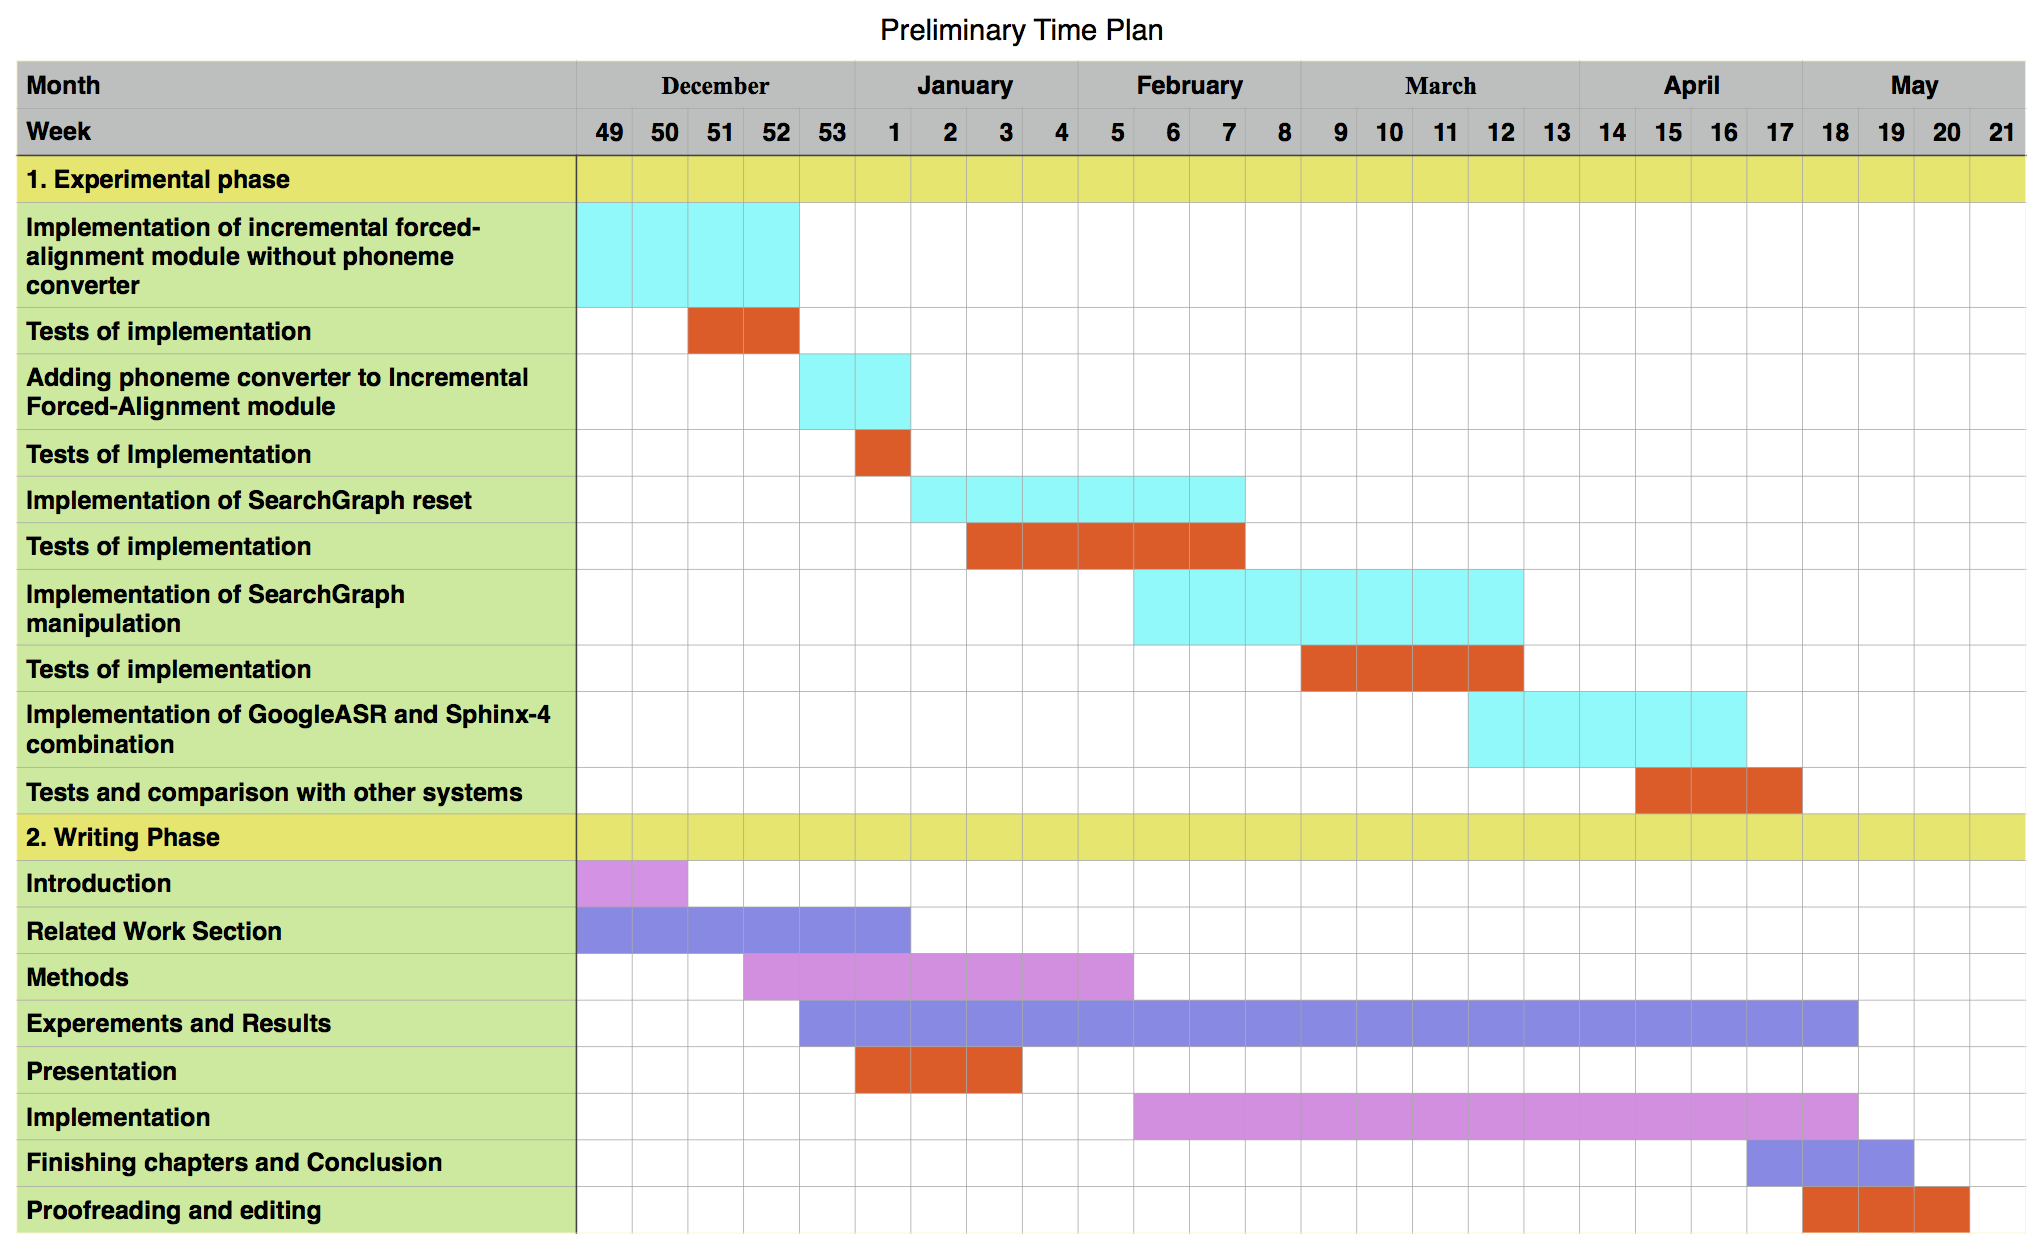
\includegraphics [width=1.2\textwidth]{images/Plan.png}
%   \caption{Preliminary timeline for the master thesis}
%   \label{fig:Bild7}
% \end{figure}
%  \end{center}
 %\end {landscape}

% \section {Conclusion}
% In this expos\'{e}  we have introduced the objectives for the upcoming master
% thesis, gave a brief literature review, formulated the research question, gave
% an overview of the methods and the test approach and present a preliminary
% table of contents and timeline for the work. In the focus of the research stays
% the possibility of latency bypassing in an incremental recogniser,
% using a combination of frontend sources and time alignment of phonemic
% representation. 


%
% EOF
%



%\include{chapters/kapitel1}
%\include{chapters/kapitel2}
%\cleardoublepage

% Anhang
%\appendix
%\include{chapters/anhang}
%\cleardoublepage
\newpage
\phantomsection % ben�tigt f�r korrekte pdf-darstellung
\addcontentsline{toc}{chapter}{References}
\printbibliography 
%\bibliographystyle{natdin} % Din 1505 nach Lorenzen (Das konkrete Aussehen des
% Litverzeichnisses ist im header festgelegt)
%\bibliography{bibliography/literatur} 
 % Pfad zur *.bib-Datei
 % (Dateiendung wird
% weggelassen)
%\cleardoublepage
%\include{_eidversicherung}
\end{document}
%